\begin{figure}[H]
\centering
\vspace{1mm}
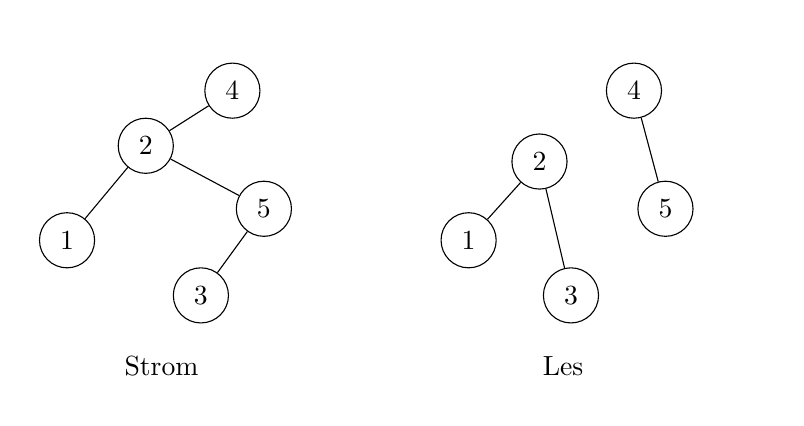
\begin{tikzpicture}[
    vnode/.style={circle, draw, minimum size=7mm, inner sep=0pt} ]
    % --- Graph (a) ---
    \node[vnode] (a2) at (0, 2) {2};
    \node[vnode] (a1) at (-1, 0.8) {1};
    \node[vnode] (a4) at (1.1, 2.7) {4};
    \node[vnode] (a5) at (1.5, 1.2) {5};
    \node[vnode] (a3) at (0.7, 0.1) {3};

    \draw (a2) -- (a1);
    \draw (a2) -- (a4);
    \draw (a2) -- (a5);
    \draw (a5) -- (a3);

    \node at (0.2, -0.8) {Strom};

    % --- Graph (b) ---
    \node[vnode] (b2) at (5, 1.8) {2};
    \node[vnode] (b1) at (4.1, 0.8) {1};
    \node[vnode] (b3) at (5.4, 0.1) {3};
    \node[vnode] (b4) at (6.2, 2.7) {4};
    \node[vnode] (b5) at (6.6, 1.2) {5};

    \draw (b2) -- (b1);
    \draw (b2) -- (b3);
    \draw (b4) -- (b5);

    \node at (5.3, -0.8) {Les};
    
    % Bounding box for padding
    \useasboundingbox (-1.5, -1.2) rectangle (8, 3.5);
\end{tikzpicture}
\vspace{0.5cm}
\caption{Obrázek stromu a lesa. Oba grafy mají 4 listy.}
\end{figure}
